\papertype{Supplementary}
% Include section in journal if known, otherwise delete
% \paperfield{Journal Section}
\title{Carbon cathodes for rechargeable aluminium-ion batteries}
% Include full affiliation details for all authors
\affil[1]{Victoria University of Wellington, School of Chemical and Physical Sciences, Wellington, New Zealand}
\affil[2]{The University of Newcastle, School of Mathematical and Physical Sciences, Callaghan, NSW 2308, Australia}
%\corraddress{Author One PhD, Department, Institution, City, State or Province, Postal Code, Country}
\corremail{thomas.nann@newcastle.edu.au}
%\presentadd[\authfn{2}]{Department, Institution, City, State or Province, Postal Code, Country}
\fundinginfo{No funding information available.}
% Include the name of the author that should appear in the running header
\runningauthor{Nann et al.}
\begin{document}
\section*{Supporting Information}
\newcommand{\beginsupplement}{
               \setcounter{figure}{0}
        \renewcommand{\thefigure}{S\arabic{figure}}
     }
\beginsupplement


\begin{figure}[tbh!]
  \centering
  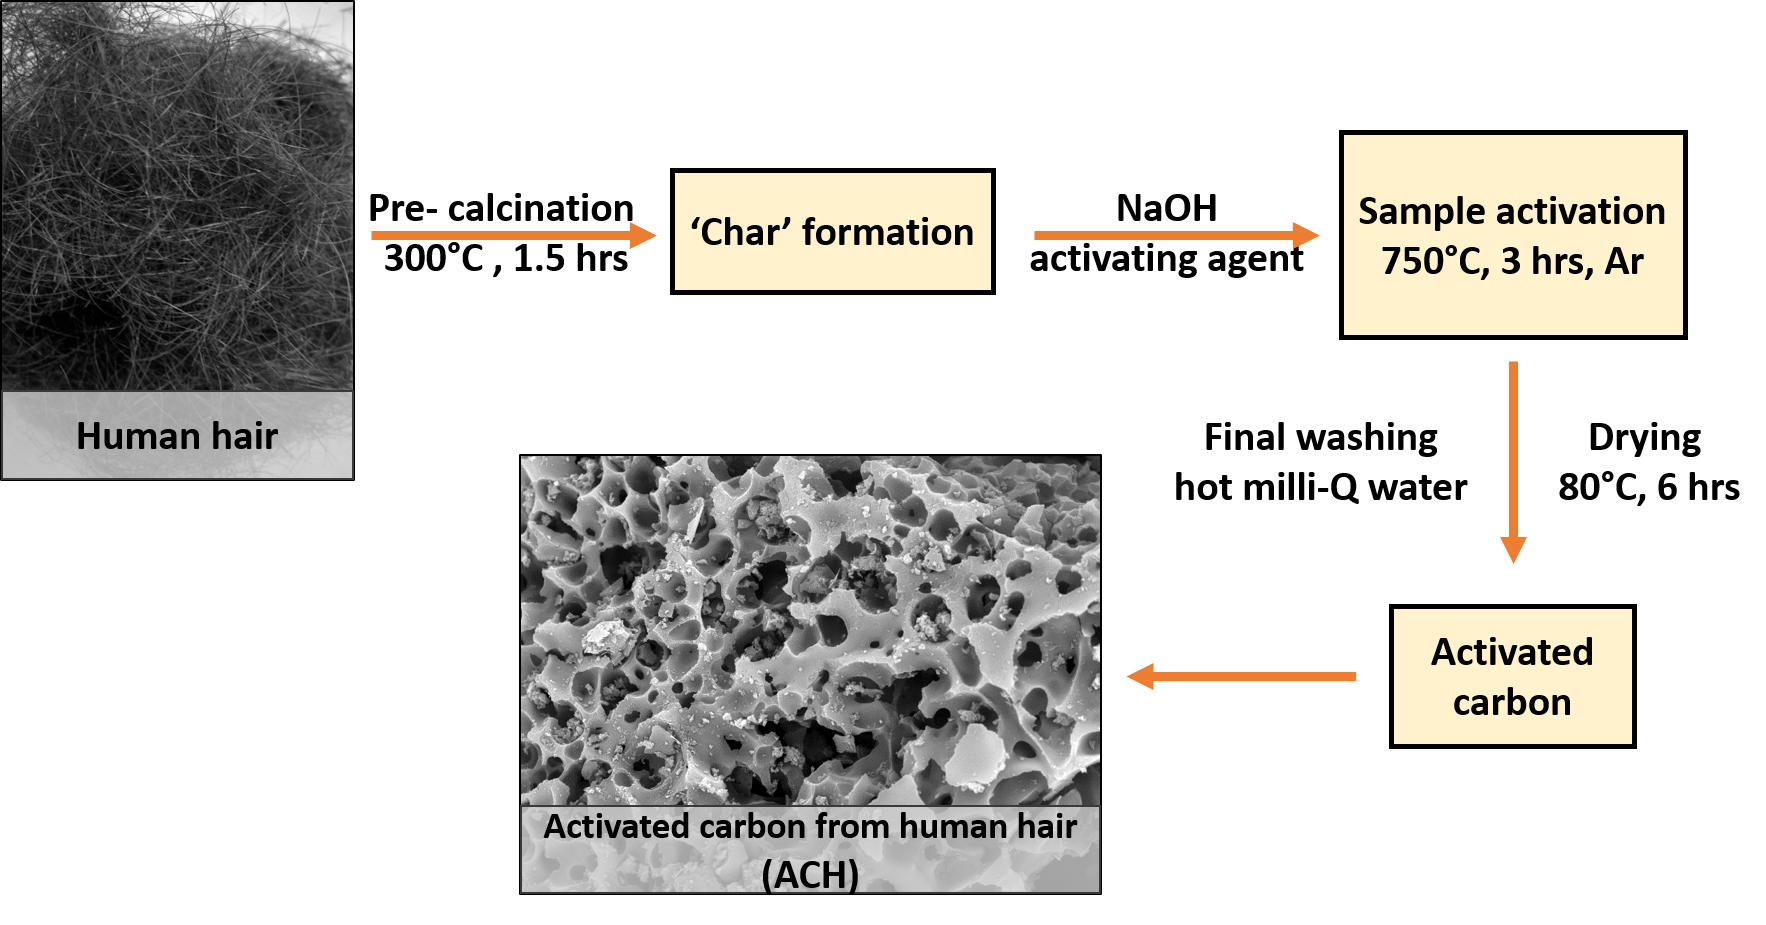
\includegraphics[width=\textwidth]{SF/ACHsyn}
    \caption{Synthesis of activated carbon from human hair using NaOH as the activating agent. The choice of temperature and activating agent plays a crucial role in determining pore size of the activated carbon.}
  \label{SF:ACHsyn}
\end{figure}
\begin{figure}[tbh!]
  \centering
  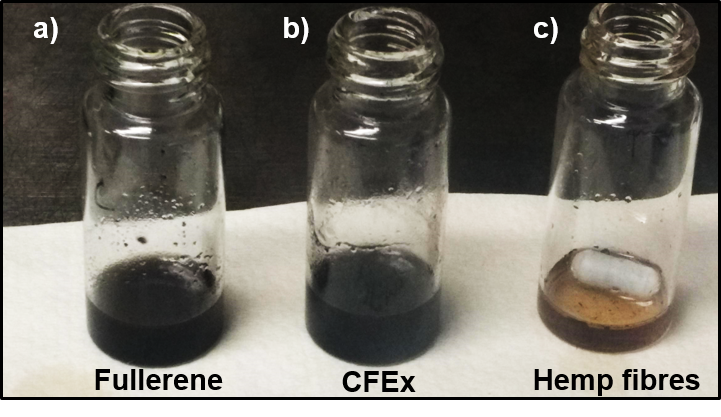
\includegraphics[width=\textwidth]{SF/CFExsol}
    \caption{Synthesis of activated carbon from human hair using NaOH as the activating agent. The choice of temperature and activating agent plays a crucial role in determining pore size of the activated carbon.}
  \label{SF:CFExsol}
\end{figure}
\begin{figure}[tbh!]
  \centering
  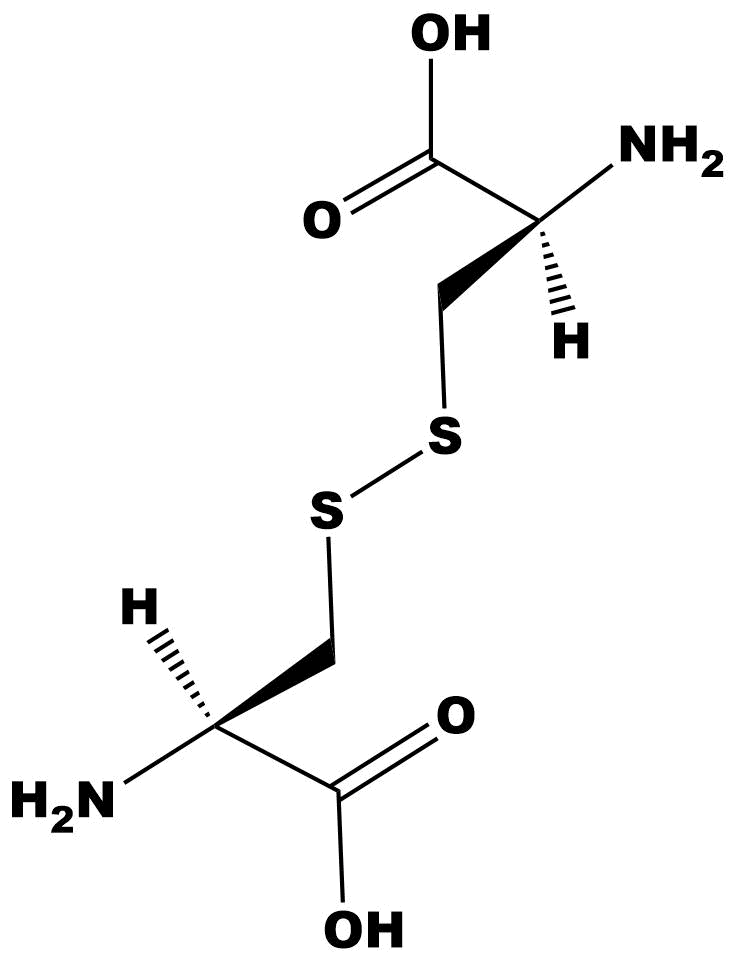
\includegraphics[width=0.5\textwidth]{SF/keratin}
    \caption{Keratin: a protein abundantly found in human hair contains C-O, C=O, C-NH$_2$ bonds.} 
    \label{SF:keratin}
\end{figure}
\begin{figure}[tbh!]
  \centering
  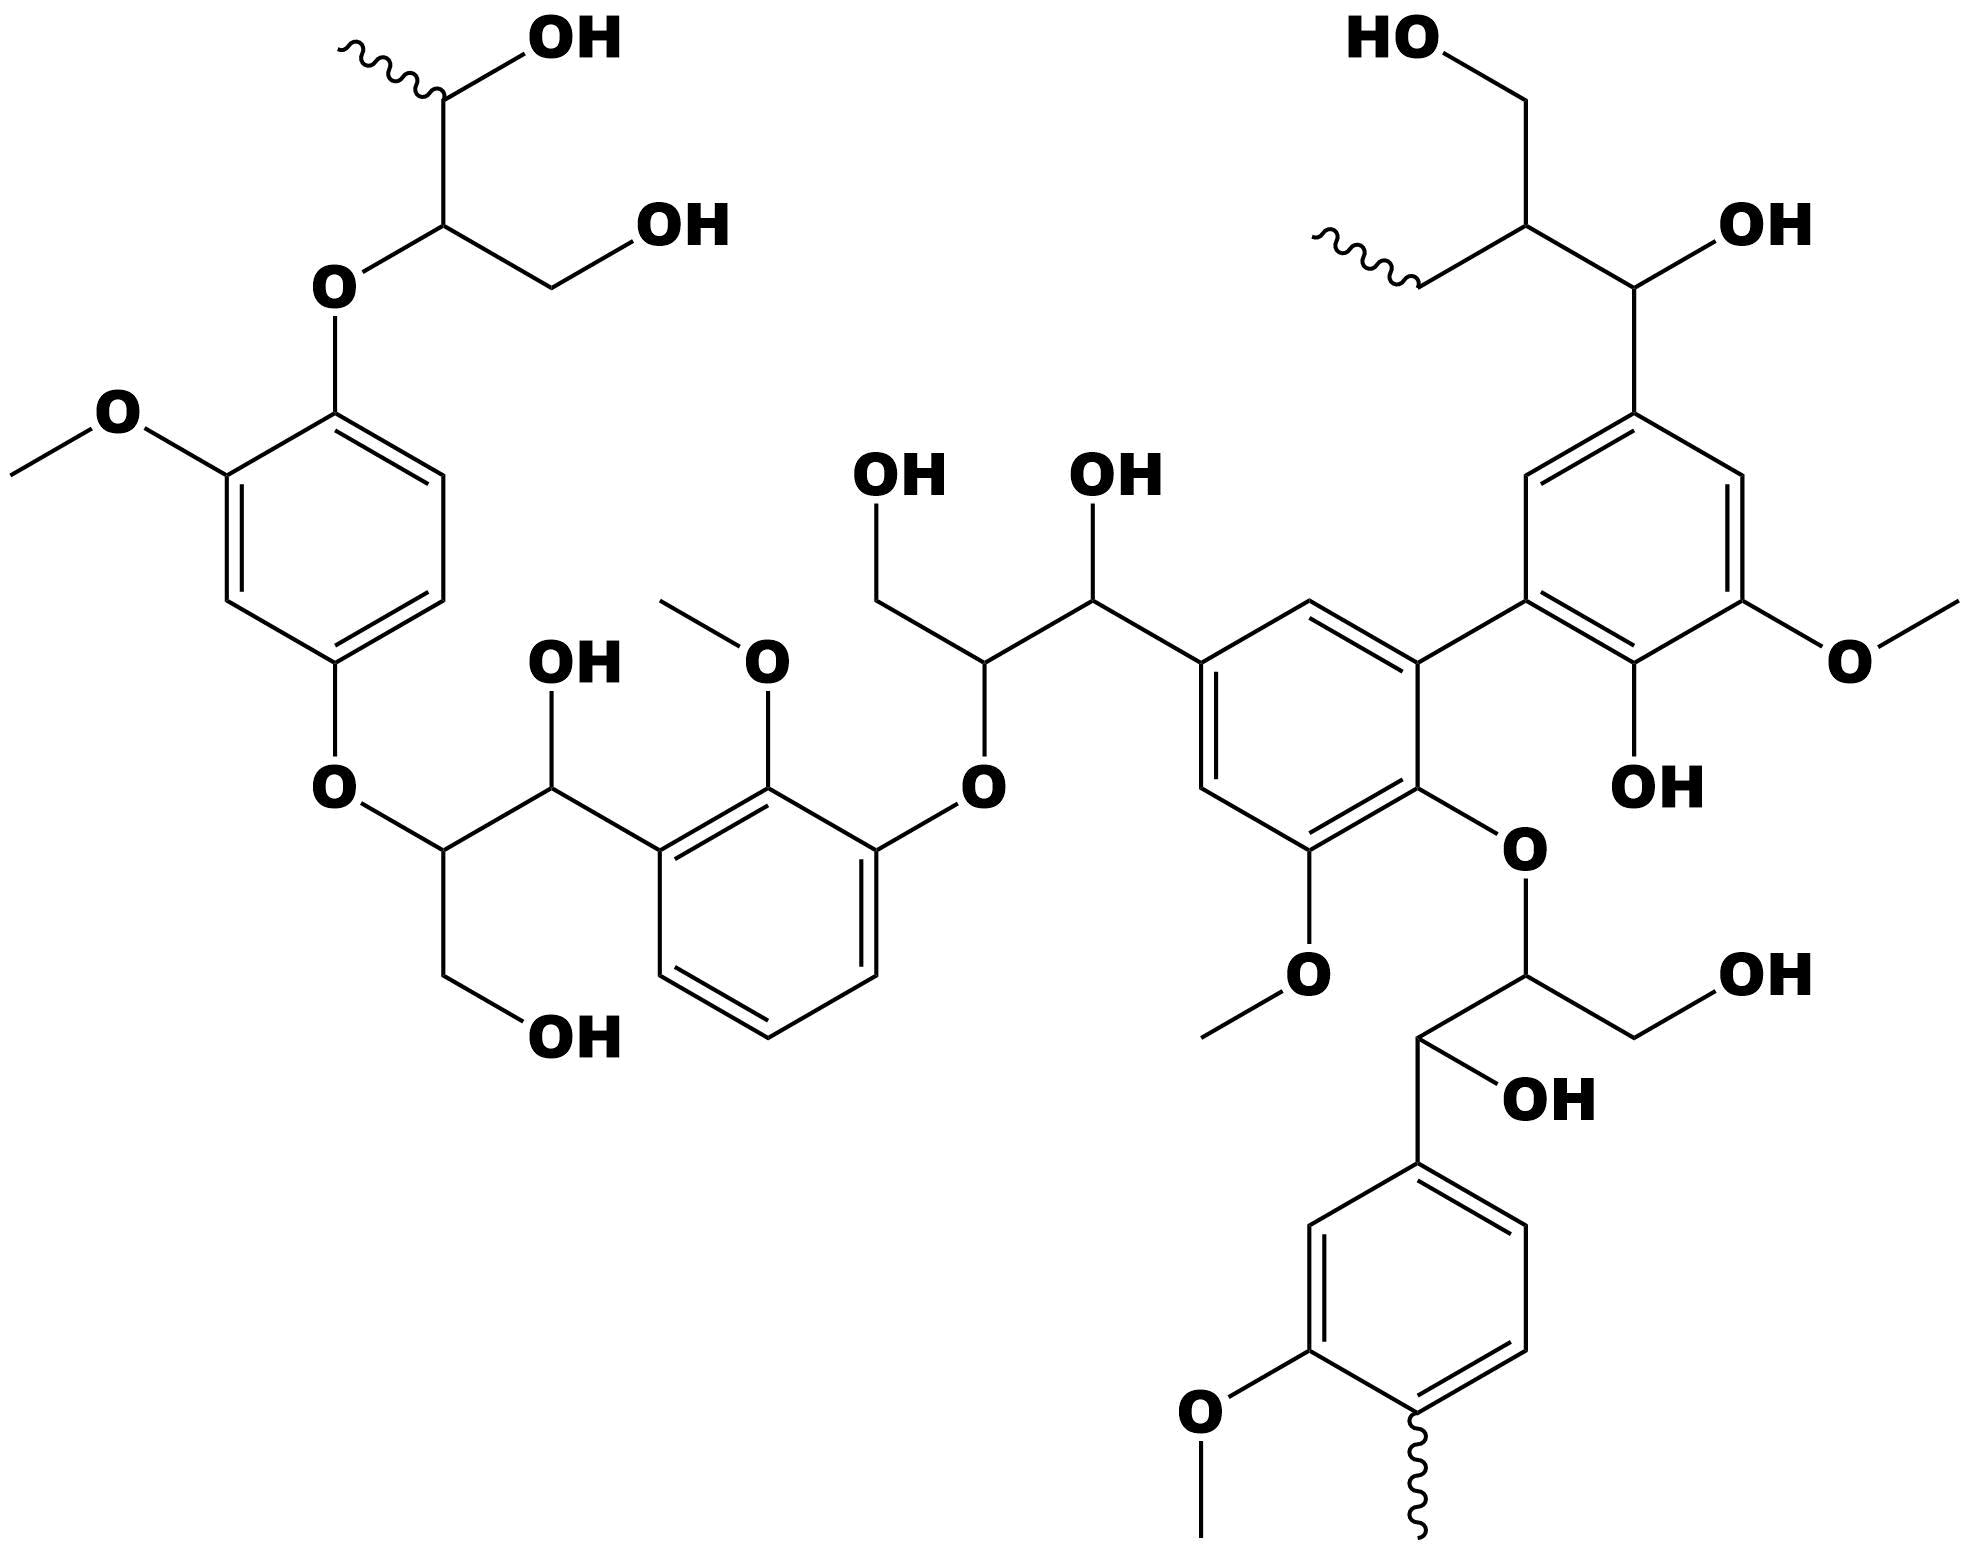
\includegraphics[width=0.5\textwidth]{SF/lignin}
    \caption{Structure of Lignin- The lignin content of hemp will vary according to the part of the plant under observation. It contains a number of carbonyl, ester groups along with other proteins such as edestin and albumin.}
  \label{SF:lignin}
\end{figure}
\begin{figure}[tbh!]
  \centering
  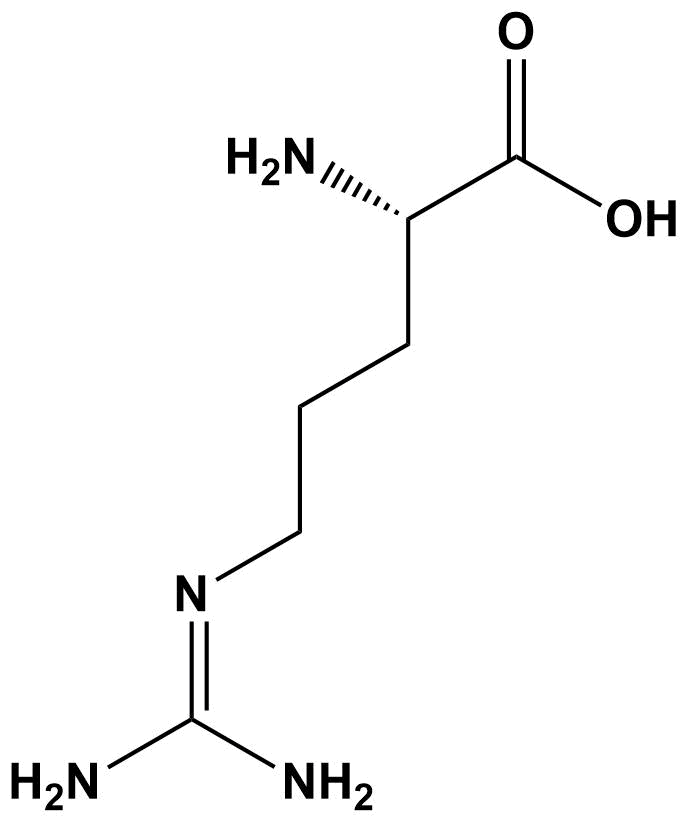
\includegraphics[width=0.5\textwidth]{SF/arginine}    \caption{Structure of Arginine- major component of hemp fibers containing C-N, C=O, C-O bonds.}
  \label{SF:arginine}
\end{figure}
\begin{figure}[tbh!]
  \centering
  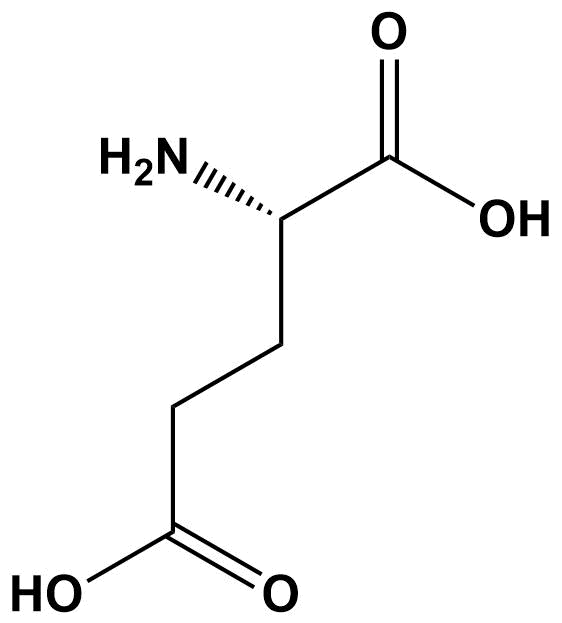
\includegraphics[width=0.5\textwidth]{SF/glutamicacid}
    \caption{Structure of Glutamic acid- another protein found in hemp fibers containing C-O, C=O and C-N bonds.}
  \label{SF:glutamicacid}
\end{figure}
\begin{figure}[tbh!]
  \centering
  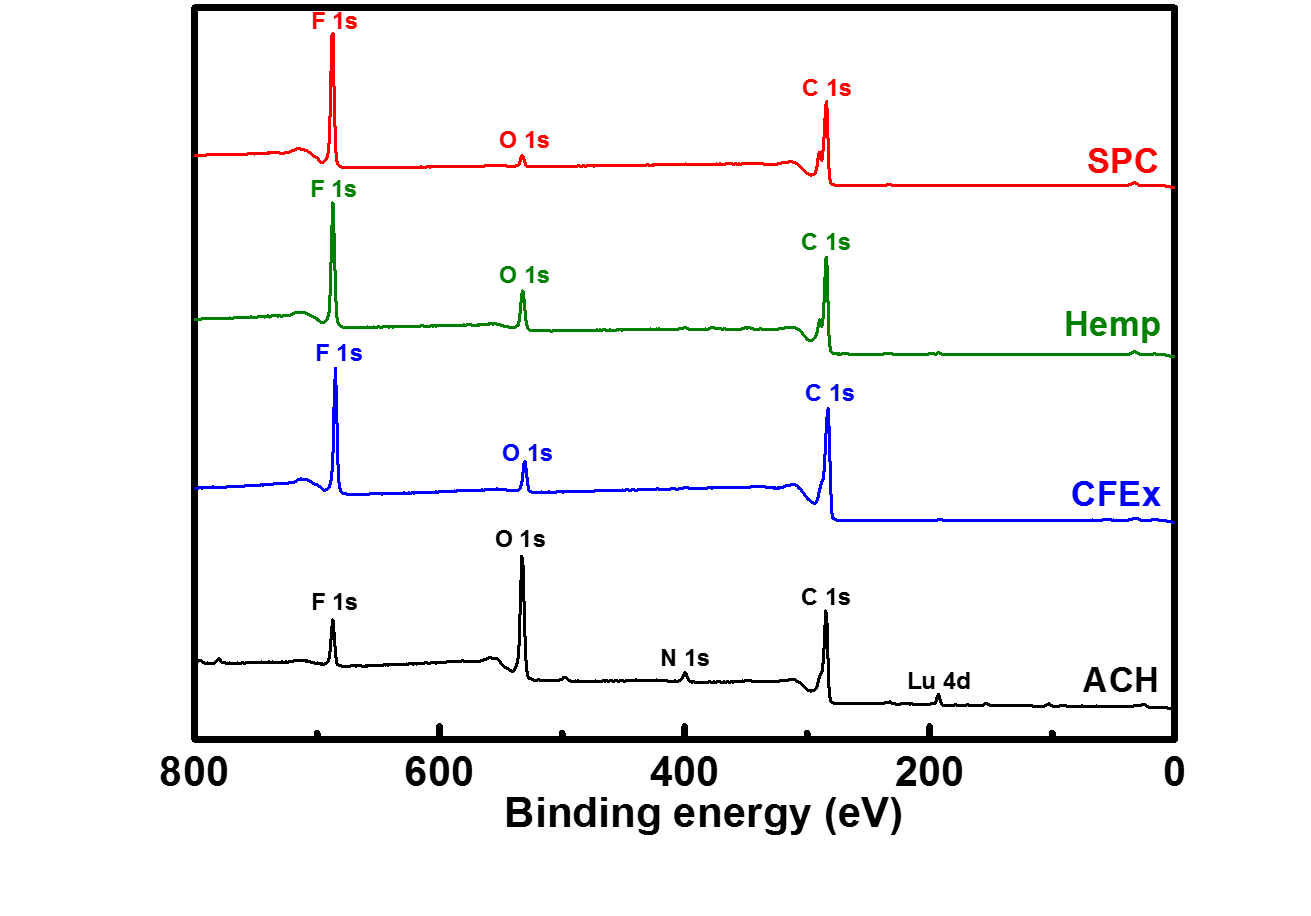
\includegraphics[width=\textwidth]{SF/XPSoverall}
    \caption{CV of ACH at a scan rate of 50 mV/s.}
  \label{SF:XPSoverall}
\end{figure}
\begin{figure}[tbh!]
  \centering
  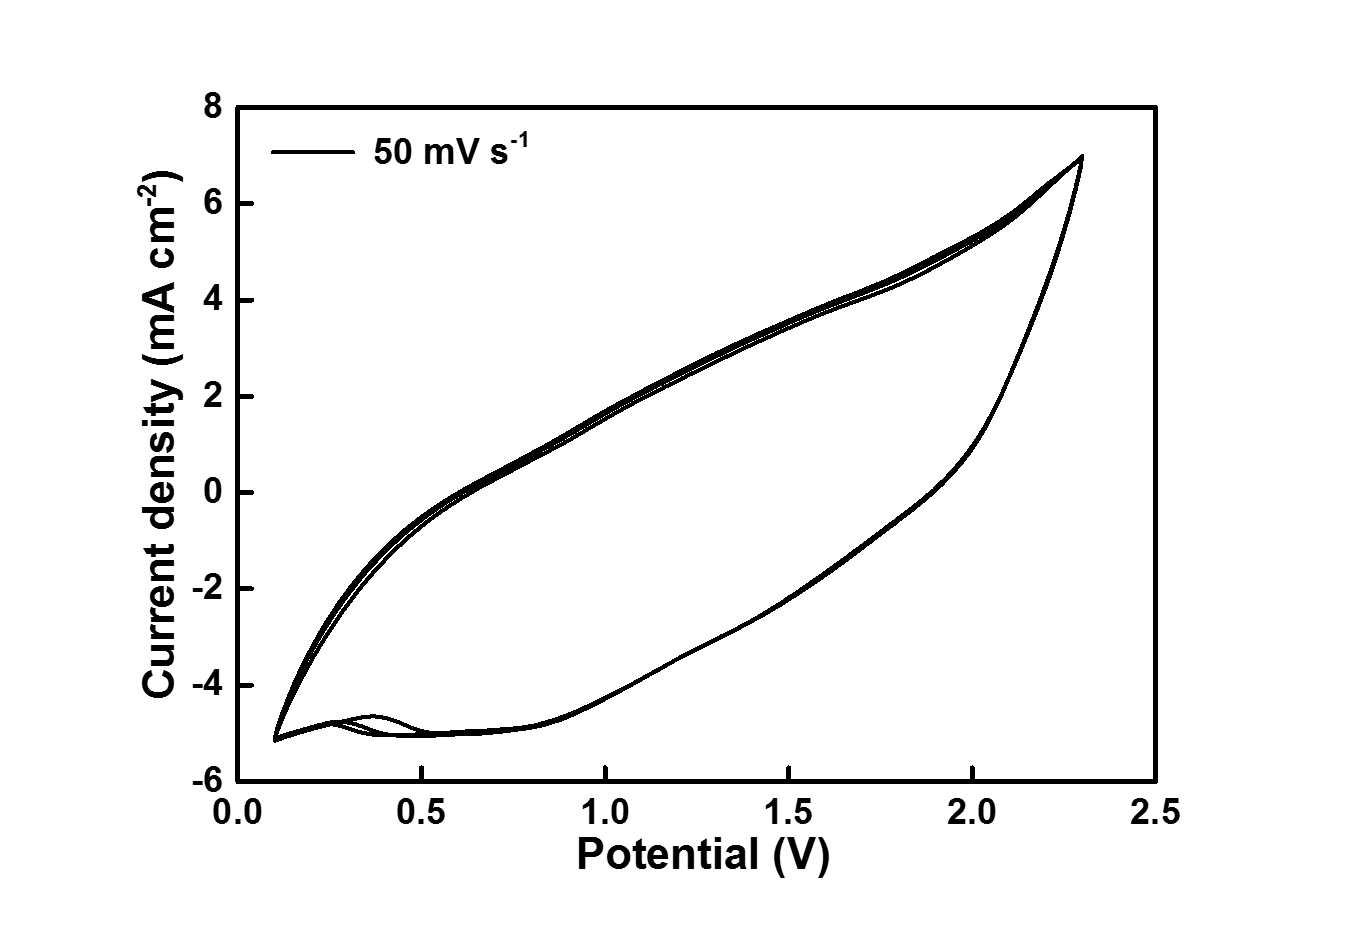
\includegraphics[width=\textwidth]{SF/hair50mVs}
    \caption{CV of ACH at a scan rate of 50 mV/s.}
  \label{SF:hair50mVs}
\end{figure}
\begin{figure}[tbh!]
  \centering
  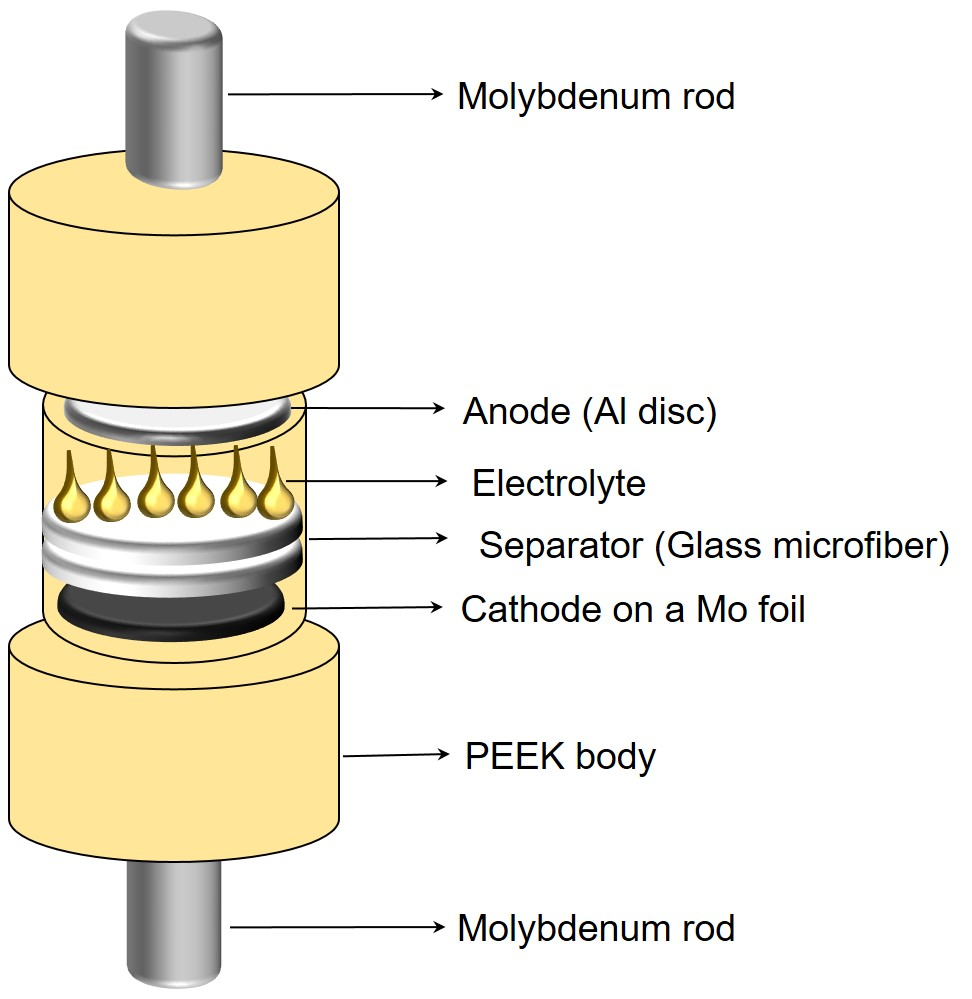
\includegraphics[width=\textwidth]{SF/PEEK}
    \caption{CV of ACH at a scan rate of 50 mV/s.}
  \label{SF:PEEK}
\end{figure}
\end{document}